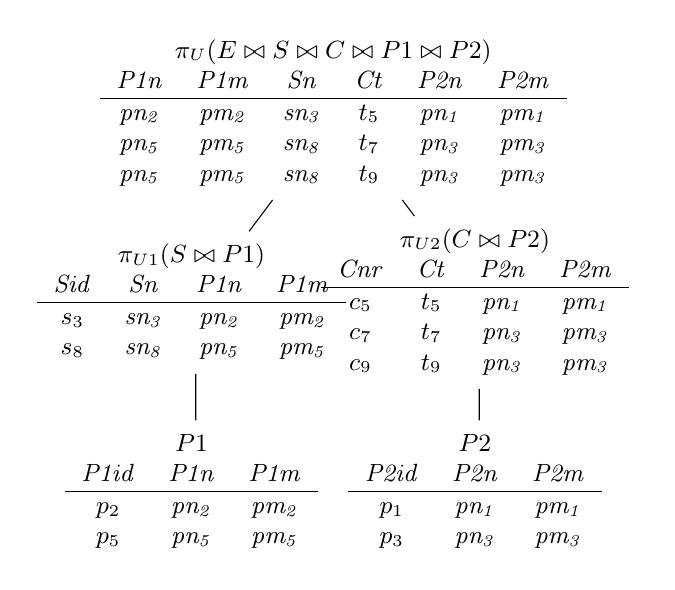
\begin{tikzpicture}[scale=0.6]
    \node	(5)	at	(-3,-4)	[align=center]	{
		\small
		\begin{tabular}{ccc}
			\multicolumn{3}{c}{$P1$}\\
			$\mathit{P1id}$ & $\mathit{P1n}$ & $\mathit{P1m}$ \\
			\hline
			$p_2$ & $\mathit{pn_2}$ & $\mathit{pm_2}$ \\
			$p_5$ & $\mathit{pn_5}$ & $\mathit{pm_5}$ \\
		\end{tabular}
	};
	\node	(4)	at	(3,-4)	[align=center]	{
		\small
		\begin{tabular}{ccc}
			\multicolumn{3}{c}{$P2$}\\
			$\mathit{P2id}$ & $\mathit{P2n}$ & $\mathit{P2m}$ \\
			\hline
			$p_1$ & $\mathit{pn_1}$ & $\mathit{pm_1}$ \\
			$p_3$ & $\mathit{pn_3}$ & $\mathit{pm_3}$ \\
		\end{tabular}
	};
	\node	(3)	at	(3,0)	[align=center]	{
		\small
		\begin{tabular}{cccc}
			\multicolumn{4}{c}{$\pi_{U2}(C \bowtie P2)$}\\
			$\mathit{Cnr}$ & $\mathit{Ct}$ & $\mathit{P2n}$ & $\mathit{P2m}$ \\
			\hline
			$c_5$ & $t_5$ & $\mathit{pn_1}$ & $\mathit{pm_1}$ \\
			$c_7$ & $t_7$ & $\mathit{pn_3}$ & $\mathit{pm_3}$ \\
			$c_9$ & $t_9$ & $\mathit{pn_3}$ & $\mathit{pm_3}$ \\
		\end{tabular}
	}
		edge(4);
	\node	(2)	at	(-3,0)	[align=center] {
		\small
		\begin{tabular}{cccc}
			\multicolumn{4}{c}{$\pi_{U1}(S \bowtie P1)$}\\
			$\mathit{Sid}$ & $\mathit{Sn}$ & $\mathit{P1n}$ & $\mathit{P1m}$ \\
			\hline
		    $s_3$ & $\mathit{sn_3}$ & $\mathit{pn_2}$ & $\mathit{pm_2}$\\
		    $s_8$ & $\mathit{sn_8}$ & $\mathit{pn_5}$ & $\mathit{pm_5}$\\
		\end{tabular}
	}
	    edge(5);
	\node	(1)	at	(0,4)		[align=center]	{
		\small
		\begin{tabular}{cccccc}
			\multicolumn{6}{c}{$\pi_U(E \bowtie S \bowtie C \bowtie P1 \bowtie P2)$}\\
			$\mathit{P1n}$ & $\mathit{P1m}$ & $\mathit{Sn}$ & $\mathit{Ct}$ & $\mathit{P2n}$ & $\mathit{P2m}$\\
			\hline
			$\mathit{pn_2}$ & $\mathit{pm_2}$ & $\mathit{sn_3}$ & $t_5$ & $\mathit{pn_1}$ & $\mathit{pm_1}$ \\
			$\mathit{pn_5}$ & $\mathit{pm_5}$ & $\mathit{sn_8}$ & $t_7$ & $\mathit{pn_3}$ & $\mathit{pm_3}$ \\
			$\mathit{pn_5}$ & $\mathit{pm_5}$ & $\mathit{sn_8}$ & $t_9$ & $\mathit{pn_3}$ & $\mathit{pm_3}$ \\
		\end{tabular}
	}
		edge(2)
		edge(3);
\end{tikzpicture}